% arara: pdflatex
% arara: pdflatex
% arara: pdflatex

% options:
% thesis=B bachelor's thesis
% thesis=M master's thesis
% czech thesis in Czech language
% slovak thesis in Slovak language
% english thesis in English language
% hidelinks remove colour boxes around hyperlinks

\documentclass[thesis=B,czech]{FITthesis}[2012/06/26]

\usepackage[utf8]{inputenc} % LaTeX source encoded as UTF-8

% My packages
\usepackage{hyperref}
\usepackage{xcolor}
\usepackage{listings}
\usepackage{minted}
\lstset{basicstyle=\ttfamily,
  showstringspaces=false,
  commentstyle=\color{red},
  keywordstyle=\color{blue}
}

\usepackage{graphicx} %graphics files inclusion
\graphicspath{ {./images/} }


% \usepackage{amsmath} %advanced maths
% \usepackage{amssymb} %additional math symbols

\usepackage{dirtree} %directory tree visualisation

% % list of acronyms
% \usepackage[acronym,nonumberlist,toc,numberedsection=autolabel]{glossaries}
% \iflanguage{czech}{\renewcommand*{\acronymname}{Seznam pou{\v z}it{\' y}ch zkratek}}{}
% \makeglossaries

\newcommand{\tg}{\mathop{\mathrm{tg}}} %cesky tangens
\newcommand{\cotg}{\mathop{\mathrm{cotg}}} %cesky cotangens

% % % % % % % % % % % % % % % % % % % % % % % % % % % % % % 
% ODTUD DAL VSE ZMENTE
% % % % % % % % % % % % % % % % % % % % % % % % % % % % % % 

\department{Katedra softewarového inženýrství}
\title{Věnná města českých královen - API~pro~předávání grafických modelů}
\authorGN{Martin} %(křestní) jméno (jména) autora
\authorFN{Čapek} %příjmení autora
\authorWithDegrees{Martin Čapek} %jméno autora včetně současných akademických titulů
\author{Martin Čapek} %jméno autora bez akademických titulů
\supervisor{Ing. Jiří Chludil}
\acknowledgements{Děkuji především své rodině za podporu, svému vedoucímu za časté konzultace a za směrování mě k práci.}
\abstractCS{Tato práce popisuje návrh a vývoj REST API pro editor virtuální reality.

První část je věnována analýze funkčním požadavkům editoru virtuální reality a nefunkčním požadavkům na API, analýze nástrojů pro návrh API a stanovení výběrové metodiky pro tyto nástroje. Z této metriky nám vyjde nejlépe ohodnocený nástroj Swagger.

V návrhové části je vytvořen doménový model databáze, který vychází ze současného stavu databáze projektu Věnná města českých královen. Funkční požadavky editoru virtuální reality jsou pokryty koncové body. Provede se návrh API s použitím nástroje Swagger a popíší se technologie potřebné pro vývoj.

Dále je popsán vývoj API, tutoriál pro vytvoření jednoduchého REST API a implementace funkčního prototypu.

Nakonec je funkční prototyp podroben automatizovaným a integračním testům.}
\abstractEN{This work describes the design and development of the REST API for the virtual reality editor.

The first part is devoted to the analysis of the functional requirements of the virtual reality editor and the non-functional requirements of the API, the analysis of API design tools and the definition of the selection methodology for these tools. This selection gives us the best rated tool Swagger.

In the design part, a domain model of the database is created, which is based on the contemporary state of the database of the project Dowry Towns of the Queens of Bohemia. The virtual reality editor's functional requirements are covered by endpoints. An API design is performed using Swagger and the technologies needed for development are described.

Next is described API development, tutorial for creating simple REST API and implementation of functional prototype.

Finally, the functional prototype is subjected to automated and integration tests.}
\placeForDeclarationOfAuthenticity{V~Praze}
\declarationOfAuthenticityOption{4} %volba Prohlášení (číslo 1-6)
\keywordsCS{vývoj API, funkční prototyp, virtuální realita, historické modely budov, Node.js, Swagger \newpage}
\keywordsEN{API development, functional prototype, virtual reality, historical models of buildings, Node.js, Swagger}
% \website{http://site.example/thesis} %volitelná URL práce, objeví se v tiráži - úplně odstraňte, nemáte-li URL práce

\begin{document}

% \newacronym{CVUT}{{\v C}VUT}{{\v C}esk{\' e} vysok{\' e} u{\v c}en{\' i} technick{\' e} v Praze}
% \newacronym{FIT}{FIT}{Fakulta informa{\v c}n{\' i}ch technologi{\' i}}

\begin{introduction}
	 Věnná města českých královen je rozsáhlý projekt, jehož cílem je vytvoření specializovaného historického průvodce věnnými městy a jejich městskou krajinou.
	 Momentálně se v tomto projektu vyvíjí editor virtuální reality, který má sloužit jako nástroj historikům a jiným odborníkům, ve kterém budou moci spolupracovat na vytváření modelů, zasazování modelů do krajiny a tím vytvářet historická věnná města. Editor umožní návštěvníkům si tato města prohlížet.

	 V mojí práci se věnuji analýze požadavků editoru virtuální reality, návrhem API pro editor, implementací jeho prototypu a otestováním prototypu.
	 
	 Uživatelé v editoru budou potřebovat API pro práci s velkým množstvím informací a garfických modelů, uložených v databázi. API bude také potřeba k~řešení přístupových práv, protože některé informace jsou citlivé a s některými modely mohou manipulovat jen lidé s příslušnými právy. 
	 
	 Výsledek této bakalářské práce bude vzorem pro vývoj API a to především pro Věnná města českých královen.
\end{introduction}

\chapter{Cíl práce}
    Cíl teoretické části práce je rozdělen na dva celky, analýzu a návrh.
	
	Analýza se provede nad funkčními a nefunkčními požadavky editoru virtuální reality. Dále se analyzují nástroje pro návrh a dokumentaci API a z těchto nástrojů se vybere nejvhodnější a s jeho použitím se navrhne prototyp API, které umožní komunikaci mezi datovým úložištěm a editorem virtuální reality. V návrhu se zaměříme na datové úložiště a způsob propagace modelů. Nakonec v návrhu popíšeme technologií, které budeme potřebovat při vývoji.

    Cílem praktické části práce je vývoj a otestování funkčního prototypu REST API za použití technologie Node.js a využítím technologie continuous integration.
	Spoučástí vývoje je postup pro přípravu vývojového prostředí a implementace funkčního prototypu.

\chapter{Analýza}
    %V této kapitole si připravím podklady pro návrh REST API. Nejdříve stanovím požadavky na API a dále vyberu nástroj pro návrh REST API.
    \section{Požadavky editoru virtuální reality}
        \subsection{Funkční} \label{sec:analFP}
            Následující sekce popisuje funkční požadavky editoru virtuální reality. To jsou požadavky, které se vztahují k funkcionalitě pro cílovou aplikaci. Tyto požadavky jsem vytvořil ve spolupráci s Patrikem Křepinským.
            
            \begin{itemize}
                \item \textbf{F1 Přihlášení} - V aplikaci musí být možnost přihlášení. Pokud se nepřihlásíte, můžete pokračovat jako host, který nemá žádná práva na grafické modely, tedy si je můžete pouze prohlížet.
                \item \textbf{F2 Odhlášení}
                
                Stejně jako přihlášení je nutná možnost odhlášení. Dále je potřeba mít možnost zůstat trvale přihlášen na tomto počítači, jinak funguje automatické odhlášení po ukončení aplikace.
               \item \textbf{F3 Práva k modelu}
               
                Model má svého autora a dále skupinu uživatelů, kteří mají některá z~následujících práv:
                \begin{itemize}
                    \item pouze čtení a zobrazení
                    \item čtení a zobrazení s možností psaní komentářů?
                    \item měnění poznámek a metadat (popis)
                    \item editace modelu
                    \item kopírování modelu pro svoje potřeby (povolení vytvořit na základě modelu jiný model)
                    \item plná práva
                \end{itemize}
                Tuto skupinu uživatelů může autor libovolně editovat. Pokud uživatel není ve skupině znamená to, že nemá žádná práva k tomuto modelu.
               \item \textbf{F4 Práva k projektu}
               
                Projekt je skupina modelů zasazená do lokace. Takovým projektem může být historický model města. Projekt má skupinu uživatelů, kteří mají některá z následujících práv:
                \begin{itemize}
                    \item Změna lokace modelu
                    \item Nahrávání
                    \item Mazání
                    \item Udělovat práva
                    \item Seskupení
                \end{itemize}
                Uživatel bude moct zařadit model do skupiny. Tato funkce poslouží k~lepší organizaci pracovního prostředí.
                \item \textbf{F5 Žádosti o práva}
                
                Dále mohou uživatelé žádat o určitá práva k modelu nebo skupině modelů a k projektu. Tuto žádost mohou autoři potvrdit.
                \item \textbf{F6 Zobrazení miniatur po přihlášení}
                
                Je třeba, aby po přihlášení měl uživatel přístup ke svým modelům. To umožní naše aplikace v podobě miniatur grafických modelů, které se po přihlášení načtou.
                \item \textbf{F7 Třídění miniatur}
                
                Tyto miniatury si bude moct uživatel třídit podle stavu modelů, přístupových práv, skupin uživatelů, atd.
                \item \textbf{F8 Zobrazení modelů projektu v určitém čase a počasí}
                
                Uživatel si bude moct zobrazit celý projekt v nějakém čase a procházet si ho. Bude si moct nastavovat počasí a denní dobu. Bude si ho moci procházet i napříč historií.
                \item \textbf{F9 Vytvoř kopii modelu}
                
                Uživatel bude moct vytvořit model na základě nějakého jiného modelu (pokud k tomu bude mít právo), aby nemusel začínat od začátku.
                \item \textbf{F10 Vytvoř nový projekt}
                
                Uživatel vytvoří prázdnou pracovní plochu, kam bude moct zasazovat modely.
                Nahrání modelu z lokálního zařízení
                Uživatel nahraje model z~disku a může ho uložit na server.
               \item \textbf{F11 Vytvoř kopii projektu}
               
                Uživatel vytvoří kopii projektu, pokud k tomu má právo, aby mohl provádět nějaké experimentální úpravy.
                \item \textbf{F12 Přidání modelu do projektu}
                
                Pokud bude moct uživatel editovat nějaký projekt, může přidávat i nové modely.
               \item \textbf{F13 Editace modelu}
               
               \begin{itemize}
                    \item smazání
                   
                    Uživatel smaže model pro který už nemá žádné využití. Po kliknutí na smazání modelu se aplikace ještě zeptá, jestli si je opravdu jist, protože grafický model může představovat desítky hodin práce a může se stát, že uživatel klikne na tlačítko smazat omylem
                    \item vytvoření
                    
                    Uživateli se zobrazí prázdná pracovní plocha, kde bude moct vymodelovat nový model.
                \end{itemize}
                \item \textbf{F14 Ulož všechny změny v projektu}
                
                Uživatel potvrdí a uloží provedené změny na server. Po tomto uložení uvidí změny všichni kdo mají k modelu přístup.
                U modelu máme dva základní typy změn:
                \begin{itemize}
                    \item transformace (rotace, translace, scale)
                    \item informace o modelu (poznámka, autorství)
                \end{itemize}
            \end{itemize}
        \subsection{Nefunkční}
            Tato sekce se zabývá nefunkčními požadavky na REST API. Tedy požadavky, které se zaměřují na nároky cílové aplikace na software a to například z hlediska bezpečnosti, spolehlivosti, či výkonu.
            \begin{itemize}
                \item \textbf{N1 Rychlost odezvy}

                    Uživatel nesmí na obdržení nebo aktualizování grafického modelu čekat. Je třeba, aby server reagoval rychle.
                \item \textbf{N2 Datová nenáročnost při komunikaci}

                    Je třeba minimalizovat množství dat posílané přes API, abychom docílili rychlosti a zbytečně nepřetěžovali spojení s koncovým uživatelem.
                \item \textbf{N3 Bezpečnost}
                    
                    Určité koncové body vyžadují oprávnění, jelikož jejich zavoláním se předávají nebo přepisují citlivá data. To se vyřeší tím, že při přihlášení dostane uživatel token, kterým se bude autorizovat u volání citlivých koncových bodů.
                \item \textbf{N4 Rozšiřitelnost}

                    API musí umožňovat případné rozšíření o další funkcionality. Také musí být řádně zdokumentováno, aby umožnilo hladší průběh rozšiřování.
                \item \textbf{N5 Použité technologie}

                    Bylo zadáno, že se bude vyvýjet v technologii Node.js za využití modulu Express.
            \end{itemize}
        \section{Nástroje pro návrh REST API}
        V této sekci provedeme výběr nejvhodnějšího nástroje, který budeme používat v další kapitole Návrh.
        Návrh API nám bude rovněž sloužit jako dokumentace, jelikož v návrhu je popsáno co API dělá a jak. Tato dokumentace slouží rozšiřitelnosti API viz nefunkční požadavek N4.
        
        Byly vybráni čtyři nejrozšířenější kandidáti, kteří nabízí své služby zdarma. Tyto kandidáty ohodnotím výběrovou metodou, ze které nám vyjde nejvhodnější nástroj pro naše potřeby.
		Výběrová metoda se bude skládat z ohodnocení nástroje z hlediska následujících metrik:
        \begin{itemize}
            \item Dokumentace nástroje
            
            	Je nutnou podmínkou, aby byl nástroj řádně zdokumentován, protože k~nástroji budu přistupovat jako laik. Tudíž veškerá funkcionalita, která nebude pokryta v dokumentaci jakoby neexistovala.
            \item Funkčnost
           	
               	Popis API záleží na specifikaci, kterou nástroje utilizují. Budu ho hodnotit třemi základními kritérii:
       	        \begin{itemize}
               	    \item Zápis koncových bodů
    		        \item Zabezpečení s JWT
    		        \item Definice objektů, které bude API předávat
        		\end{itemize}
    	        Dále by návrh API měl jít vizualizovat do podoby čitelné dokumentace.
            \item GitHub repozitář
            
                Na repozitář se budeme dívat z ohledu oblíbenosti (na GitHubu mohou uživatelé dávat hvězdičky repozitářům), posledních commitů a řešených problémů
            \item Fórum
            
                Můžeme narazit na různé problémy, které lze vyřešit na fóru, nebo najít konverzaci na fóru s podobnou tématikou. Budeme tedy hodnotit jak je fórum obsáhlé a jak je živé (poslední příspěvek, rychlost odpovědí).
        \end{itemize}
        Popíši každý z vybraných nástrojů a ohodnotím je z pohledu vybraných metrik a na konec dám samostatně metriku GitHub repozitáře.
        \subsection{Swagger}
            Swagger \cite{swagger} je sada nástrojů postavená na OpenAPI Specifikaci. OpenAPI Specifikace, dřívěji Swagger Specifikace, je sada pravidel, které sémanticky popisují API. Nástroje:
            \begin{itemize}
                \item Swagger editor - editor umožňující psát OpenAPI Specifikaci
                \item Swagger UI - vizualizuje API dokumentaci
                \item Swagger Codegen - vygeneruje kód clientské nebo serverové části
            \end{itemize}
            Metriky:
            \begin{itemize}
                \item Dokumentace
                
                    Dokumentace je rozsáhlá. Abyste mohli psát dokumentaci pro API ve~Swaggeru, musíte ovládat OpenAPI Specifikaci. Ta je zde detailně popsána a při jejím čtení jsem si připadal jako když se učím nový programovací jazyk (jsou zde popsány datové typy, dědění a polymorfismus). Dále je zde obsáhlá dokumentace SwaggerHubu, což je webová aplikace, která přináší všechny základní vlastonsi Swaggeru. Dokumentace má tutoriály a díky SwaggerHubu si je můžete rovnou vyzkoušet.
                \item Funkčnost
                
                    Splňuje požadovanou funkčnost.
                \item Fórum
                
                    Fórum\footnote{\url{https://community.smartbear.com/t5/Swagger-Open-Source-Tools/bd-p/SwaggerOSTools}} je aktivní a má i GitHub Issues.
            \end{itemize}
        \subsection{Apicurio Studio}
            Apicurio Studio \cite{apicur} je open-source editor pro OpenAPI specifikaci. Musíte se přihlásit a vaše návrhy REST API se ukládají do vašeho repozitáře na GitHubu, GitLabu nebo Bitbucketu, což se hodí v případě, když na návrhu pracujete spolčně v týmu. V editoru můžete přepínat mezi interaktivní vizualizací návrhu a jeho JSON/YAML definicí.
            \begin{itemize}
                \item Dokumentace
                
                    Dokumentace není nijak obsáhlá a není z ní zjevné, co tento nástroj dokáže a co naopak neumí. Odkaz na vyzkoušení online verze editoru nefungoval (chyba DNS\_PROBE\_FINISHED\_NXDOMAIN).
                \item Funkčnost
                
                    Splňuje požadovanou funkčnost.
                \item Fórum
                
                    Fórum pouze v podobě GitHub Issues.
            \end{itemize}
        \subsection{API Workbench}
            \href{http://apiworkbench.com}{API Workbench} \cite{apiworkbench}, narozdíl od výše zmíněných nástrojů, pracuje s RAML. RAML je akronym RESTful API Modeling Language a je to typ souboru podobný YAML, který specifikuje návrh API. API Workbench je v beta verzi a funguje jako balíček pro Atom, což je textový editor.
            
            \begin{itemize}
                \item Dokumentace
                
                    Dokumentace je stručná, přehledná, výstižná. Obasahuje tutoriál jak si napsat návrh pro jednoduché API, ale není zde vidět jak vypadá vizualizovaný návrh. Pro vizualizaci si musíte nainstalovat další nástroj \href{https://github.com/mulesoft/api-designer}{API Designer}.
                \item Funkčnost
                
                    Splňuje požadovanou funkčnost.
                \item Fórum
                
                    Fórum\footnote{\url{https://community.smartbear.com/t5/Swagger-Open-Source-Tools/bd-p/SwaggerOSTools}} je aktivní a má i GitHub Issues.       
            \end{itemize}
        \subsection{Apiary}
            Apiary \cite{apiary} editor je založen na API Blueprint, což je podobně jako OpenAPI Specifikace sada pravidel popisující API. API Blueprint specifikace má vlastní formát APIB, který má syntaxi podobnou Markdownu a využívá MSON\footnote{\url{https://github.com/apiaryio/mson}}.
            Apiary disponuje interaktivní dokumentací, webový editor má možnost přepnutí do tmavého režimu. Dále zajišťuje propojení s GitHub repozitářem.
            \begin{itemize}
                \item Dokumentace
                
                    Dokumnetace pro apiary editor je jedna stránka bez tutoriálu. Obsahuje jak vypadá editor, popis základní funkcionality a seznam klávesových zkratek. Má tedy nejmenší dokumentaci ze všech hodnocených nástrojů.
                \item Funkčnost
                
                    Splňuje požadovanou funkčnost.
                \item Fórum
                
                    Nic jako fórum jsem nenašel, pouze FAQ.
            \end{itemize}
        \subsection{GitHub repozitář}
            Metriku GitHub repozitář jsem zapsal do \hyperref[tab:tabulkaPokryti]{tabulky 2.1}.
            Nástroj Apiary nemá GitHub repozitář, tudíž ho nemůžu hodnotit. U Swaggeru jsem hodnotil jak repozitář pro editor tak pro UI a to tím způsobem, že hvězdičky jsem zprůměroval, poslední commit je nejposlednejší commit obou repozitářů a Issues jsem sečetl. Data jsou ze dne 14.4.2019.
            \begin{table}[h!]
            	\caption{Metrika GitHub repozitáře \cite{githubSwaggerUI, githubSwaggerEditor, githubApicur, githubApiworkbench}} \label{tabulkaMatrikyGitHub}
            	\begin{tabular}{| p{3cm} | p{2cm} | p{5cm} | p{2cm} |}  \hline
            		 & Swagger & Apicurio Studio & API Workbench
            		\tabularnewline \hline \hline
                    Hvězdičky & 9 799 & 310 & 219
                	\tabularnewline \hline
                    Poslední commit & 14.4.2019 & 12.4.2019 & 3.4.2018
                	\tabularnewline \hline
                    \parbox[t]{3cm}{Issues \\otevřené/uzavřené} & 417/4723 & 153/456 & 133/350
                	\tabularnewline \hline
                    Další poznámky & & Smíšené ruzné jazyky - JavaScript 32.7\%, Java 30.9\%, TypeScript 22.9\% &
                	\tabularnewline \hline
                \end{tabular}
            \end{table}
            \newline
            Swagger repozitář je tedy nejpopulárnější a nejživější (časté commity, rozsáhlé issues)
        \subsection{Výsledek výběru nástroje pro návrh API}
            Vítězem tohoto pomyslného souboje se stal \textbf{Swagger}. Vyhrál v kategoriích Dokumentace a GitHub repozitář. Fórum vyhovoje naším požadavkům a fukcionalitu splnily všechny nástroje.
\chapter{Návrh}
    V této kapitole provedu návrh REST API na základě \hyperref[sec:analFP]{analýzy funkčních požadavků}. Obecný průběh volání API je zobrazen na \hyperref[fig:volaniAPI]{obrázku 3.1}.
    \begin{figure}[h!] \label{volaniAPI}
        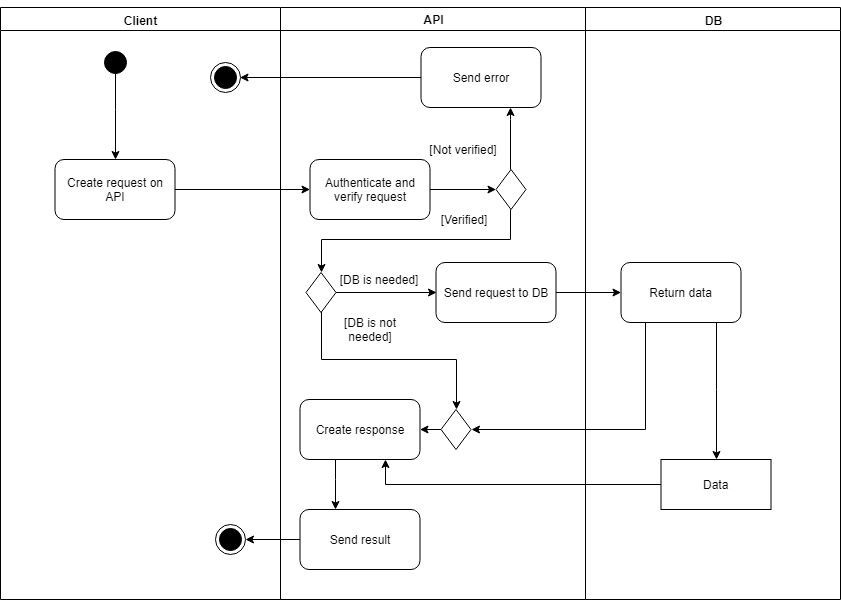
\includegraphics[width=\linewidth]{API_call}
        \caption{Proces volání API}
    \end{figure}
    
    Z obrázku je patrné, že API musí znát databázi, aby na ní mohlo vytvářet požadavky, a editor musí znát naše API, aby ho mohl správně volat. Databáze projektu Věnná města českých královen je zachycena na \hyperref[fig:volaniAPI]{obrázku 3.2}.

    \begin{figure}[h!] \label{soucasnaDB}
        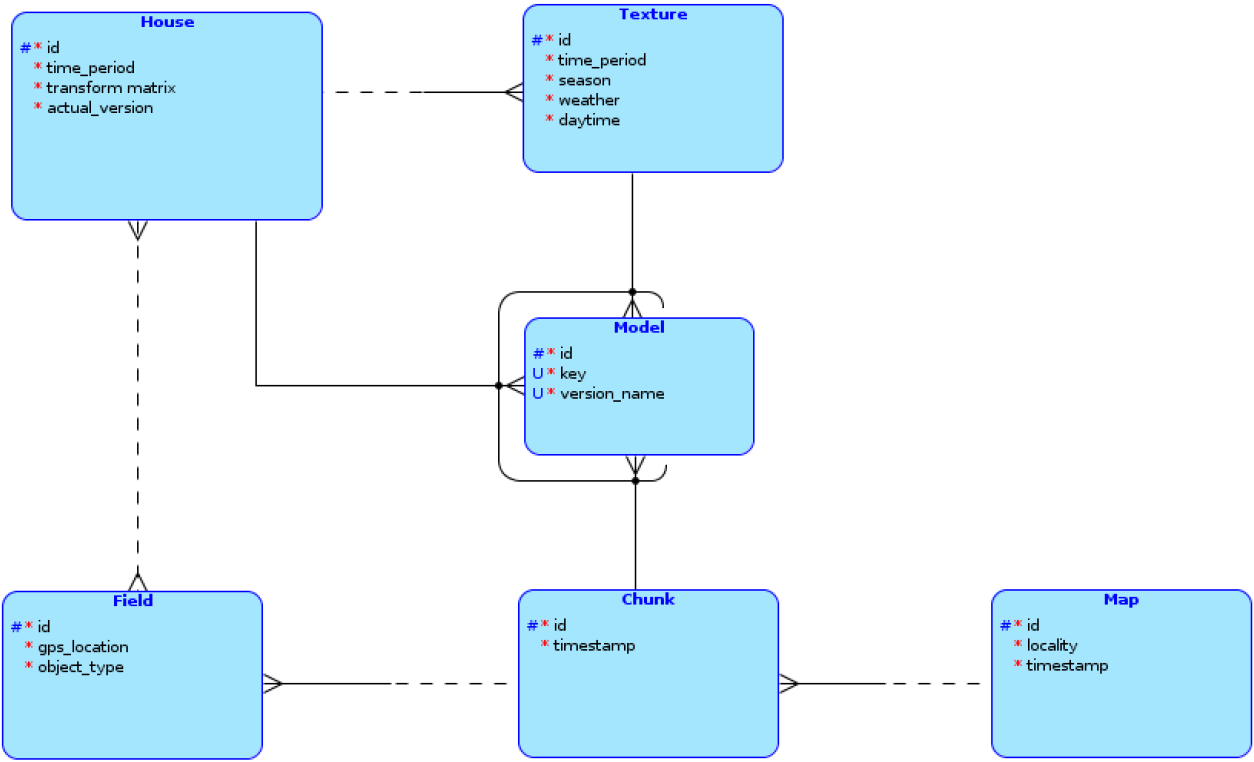
\includegraphics[width=\linewidth]{contemporary_database}
        \caption{Současná databáze}
    \end{figure}
    \newpage
    Nacházíme se ve stavu, kdy známe schéma databáze i jak vypadají požadavky na API, takže nám nic nebrání v jejím návrhu. Předem se ale musíme ujistit, že databázové schéma pokrývá požadavky.
    
    \section{Srovnání databáze s požadavky}
        Editor virtuální reality požaduje správu práv a uživatelských účtů. Tuto funkcionalitu momentálně datová vrstva nepodporuje. Navíc editor virtuální reality nepotřebuje entitu Chunk a tato entita návrh zbytečně komlikuje.
        Bude tedy potřeba provést změnu v databázovém schématu pro plnou podporu Editoru.
        Byl vytvořen doménový model pro databázi, který pokrývá požadavky Editoru, znázorněný na \hyperref[fig:domainModel]{obrázku 3.3}. Realizátoři datové vrstvy Věnných městech českých královen se budou muset rozhodnout, zda databáze pro editor virtuální reality bude existovat vedle současné datbáze, nebo provedou integraci databází.
        \begin{figure}[h!] \label{domainModel}
            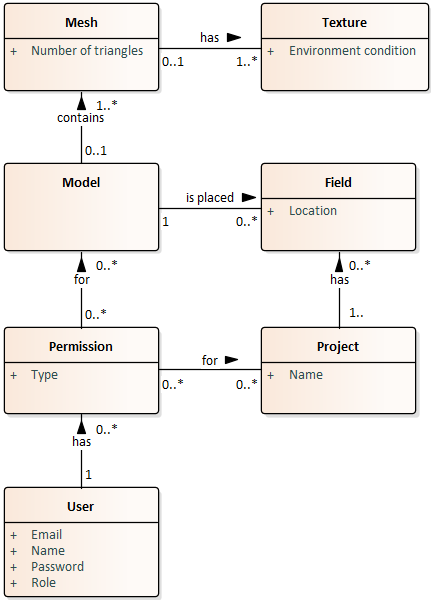
\includegraphics[width=\linewidth]{Domain_model}
            \caption{Doménový model}
        \end{figure}
        \newline
        Vysvětlení jednotlivých tabulek \hyperref[fig:domainModel]{obrázku 3.3}:
        \begin{itemize}
            \item Model
            
            Model je grafický model.
            \item Field
            
            Field reprezentuje umístění objektu. Snadno si ho lze představit jako půdorys.
            \item Project
            
            Projekt reprezentuje kolekci Fieldů, tedy zasazení grafických modelů. Může se jednat například o město v určitém historickém období.
            \item User
            
            User, nebo--li uživatel, je někdo, kdo vytváří či upravuje grafické modely nebo zasazuje a upravuje pozici modelů v projektu.
            \item Permission
            
            Aby uživatel mohl pracovat s modely a projekty musí k nim mít příslušná práva.
            \item Mesh
            
            Polygon mesh (doslovně přeloženo jako \uv{polygonální síť}) se používá v počítačové grafice a reprezentuje tvar objektu. Je to soubor vrcholů, hran a povrchů, které dohromady vytváří mnohostěn.
            \item Texture
            
            Textura jednotlivého domu. Předpokládáme textury pro různá počasí, různé roční období, různé denní doby apod.
        \end{itemize}
        Tento doménový model bude inspirací pro můj návrh API a jeho implementaci.
    \section{Pokrytí funkčních požadavků}
        Pokrytí funkčních požadavků jsem zachytil v \hyperref[tab:tabulkaPokryti]{tabulce 3.1}, kde ke každému požadavku je uveden koncový bod API, zapsaný syntaxí používanou ve Swaggeru. Funkční požadavky Odhlášení a Třídění miniatur nebudeme řešit v~tomto návrhu, protože se o ně postará Editor.
        Odhlášení se provede v aplikaci odstraněním \hyperref[sec:jwt]{JWT}.
        Třídění miniatur následuje po Zobrazení miniatur, miniatury tedy budou uloženy v aplikaci a o jejich třídení se postará aplikace.
    
        \begin{table}[h!]
        	\caption{Pokrytí funkčních požadavků} \label{tabulkaPokryti}
        	\begin{tabular}{| p{6cm} | p{6cm} |}\hline
        		Funkční požadavek & API endpoint
        		\tabularnewline \hline \hline
                Přihlášení & GET /login
            	\tabularnewline \hline
                Smaž model &	DELETE /model/\{modelId\}
            	\tabularnewline \hline
                Vytvoř nový model &	PUT /model
            	\tabularnewline \hline
                Editovat práva k modelu & POST /permission/\{permissionId\} /model/\{modelId\}
            	\tabularnewline \hline
                Editovat práva k projektu &	POST /permission/\{permissionId\} /project/\{projectlId\}
            	\tabularnewline \hline
                Seskupení & POST /group/\{groupId\}
            	\tabularnewline \hline
                Žádosti o práva & GET~/rights/model/ \{modelId\}
            	\tabularnewline \hline
                Zobrazení miniatur po přihlášení & GET /models
            	\tabularnewline \hline
                Zobrazení modelů projektu v určitém čase a počasí &
                \parbox[t]{6cm}{GET /model/\{modelId\}/time/\\\{time\}/weather/\{weather\}}
            	\tabularnewline \hline
                Ulož všechny změny v projektu &	POST /project/\{projectlId\}
            	\tabularnewline \hline
                Vytvoř kopii modelu	& PUT /model
            	\tabularnewline \hline
                Přidání modelu do projektu & POST /project/\{projectlId\}
            	\tabularnewline \hline
                Vytvoř nový projekt & PUT /project
            	\tabularnewline \hline
                Vytvoř kopii projektu &	PUT /project
            	\tabularnewline \hline
                Nahrání modelu z lokálního zařízení & PUT /project
            	\tabularnewline \hline
            \end{tabular}
        \end{table}
    \newpage
    \section{Návrh ve Swaggeru}
        Na základě \hyperref[tab:tabulkaPokryti]{tabulky 3.1} jsem vytvořil návrh ve Swaggeru. Uvedu zde příklad zapsání jednoho koncového bodu, zbytek najdete v elektronické příloze docs. Na \hyperref[fig:SwaggerYAML]{obrázku 3.4} je zapsaný koncový bod v OpenAPI Specifikaci a na \hyperref[fig:SwaggerGenerated]{obrázku 3.5} je vidět jeho vizualizace.
        \begin{figure}[h!] \label{SwaggerYAML}
            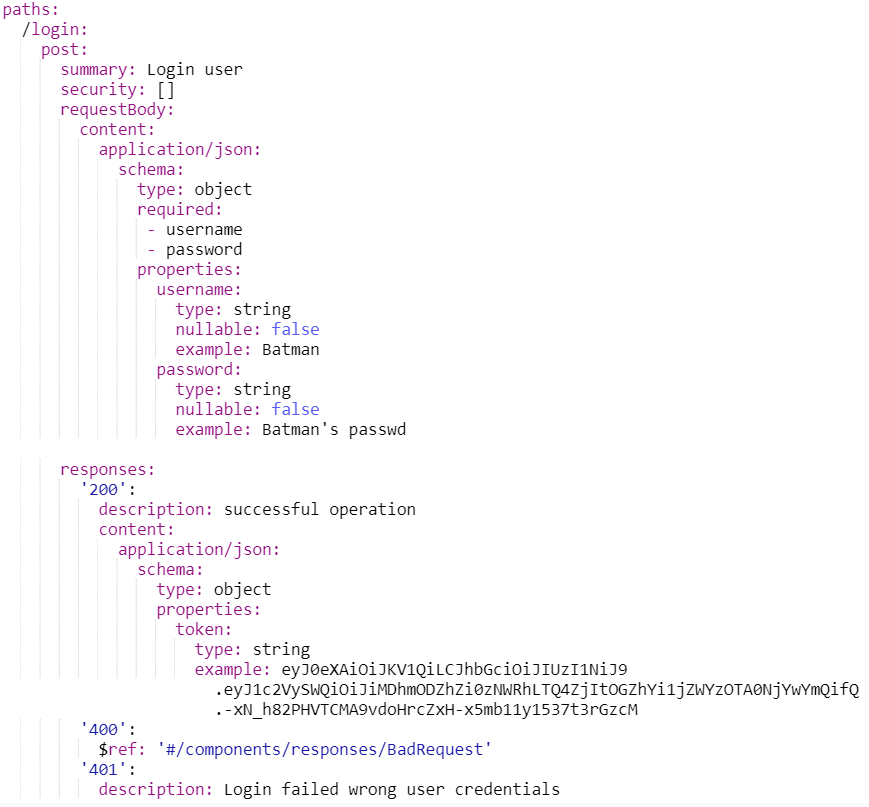
\includegraphics[width=\linewidth]{Swagger_YAML_example}
            \caption{Popis koncového bodu ve Swaggeru}
        \end{figure}
        \begin{figure}[h!] \label{SwaggerGenerated}
            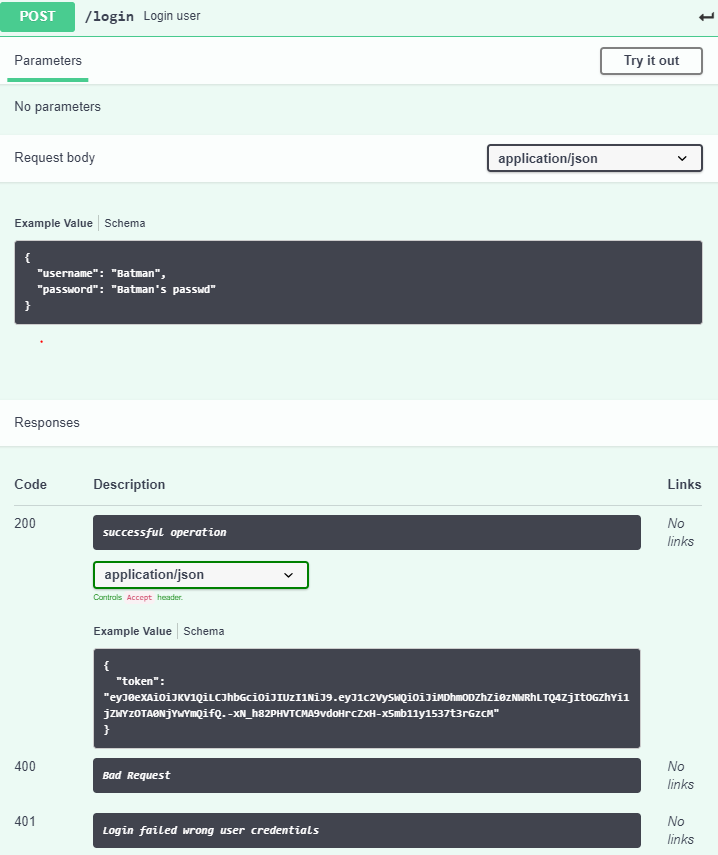
\includegraphics[width=\linewidth]{Swagger_generated_example}
            \caption{Vygenerovaný koncový bod ve Swaggeru}
        \end{figure} 

    \section{Použité technologie}
     Zde se budu věnovat technologiím, které použiji při vývoji API.
        \subsection{Rest API}
        REST, neboli Representional State Transfer, je architektonický styl, který umožňuje přistupovat k datům a využívá již existující HTTP. REST implementuje čtyři základní metody, známé pod akronymem CRUD, jsou to
        Create (vytvoření dat), Retrieve (získání požadovaných dat), Update (změnu) a Delete (smazání). Dokáže vracet XML, JSON, YAML nebo jiné formáty podle klientových požadavků. \cite{rest}
        
        V naší implementaci budeme používat JSON, jelikož se používá ve Věnných městech českých královen.
        \subsection{Node.js}
            Node.js je open-source multiplatformní JavaScriptové prostředí postaveno na Chrome V8 JavaScript enginu. Primární účel Node.js je tvorba serverové části webových aplikací, které vychází z paradigmatu \uv{JavaScript everywhere}.
            
            Node.js využívá událostmi řízenou architekturu a neblokující I/O operace. Tento návrh optimalizuje výkon a škálovatelnost programů s častými požadavky na I/O operace.
            
            Jádro celého Node.js tvoří smyčka událostí, která běží na jednom vlákně. Ta podporuje desetitisíce souběžných připojení bez nutnosti neustálého přepínání kontextu díky neblokujícímu I/O. Nedochází zde k žádnému zamykání, tudíž nemusíme mít obavy z deadlocku systému.
            \cite{node}
        \subsection{Implementační jazyk}
            Pro vývoj byl vybrán jazyk TypeScript, který je kompilovatelný do JavaScriptu. Tento jazyk je vyvýjen firmou Microsoft a jeho hlavní myšlenkou je být nadstavbou JavaScriptu, která přidává statické typování a další funkcionalitu.
        \subsection{PostgreSQL}
            Realizátory datové vrstvy v projektu Věnná města českých královen byla vybrána databáze PostgreSQL.
            
            PostgreSQL je objektově-relační databázový systém pod MIT licencí. Je pověstný svou spolehlivostí a vysokou bezpečností. Na PostgreSQL wiki\footnote{\url{https://wiki.postgresql.org/wiki/Community_Guide_to_PostgreSQL_GUI_Tools}} lze nalézt rozsáhlý seznam dostupného open-source software, sloužícího k administraci a monitoringu PostgreSQL databází. Nejrozšířenější a velmi přehledný je pgAdmin.
            \cite{postgres}
        \subsection{npm}
            Node.js využívá správce balíčků npm, jehož pomocí můžeme obecně instalovat i spravovat závislosti a spouštět skripty. Npm se chlubí tím, že je největším balíčkovacím správcem a aktuálně obsahuje skoro 800 000 balíčků.
            \cite{modulecounts}
        \subsection{Express}
            Express je framework pro Node.js, který nám umožnuje jednoduše napsat webovou aplikaci, či API. Těší se velké popularitě a podle \cite{npmrank} je na něm závislých 21 873 balíčků.
        \subsection{JWT} \label{jwt}
            JWT (JSON Web Token) je standart, který zajišťuje bezpečný přesun informací zapsaných v JSON.
            \begin{figure}[h!]
                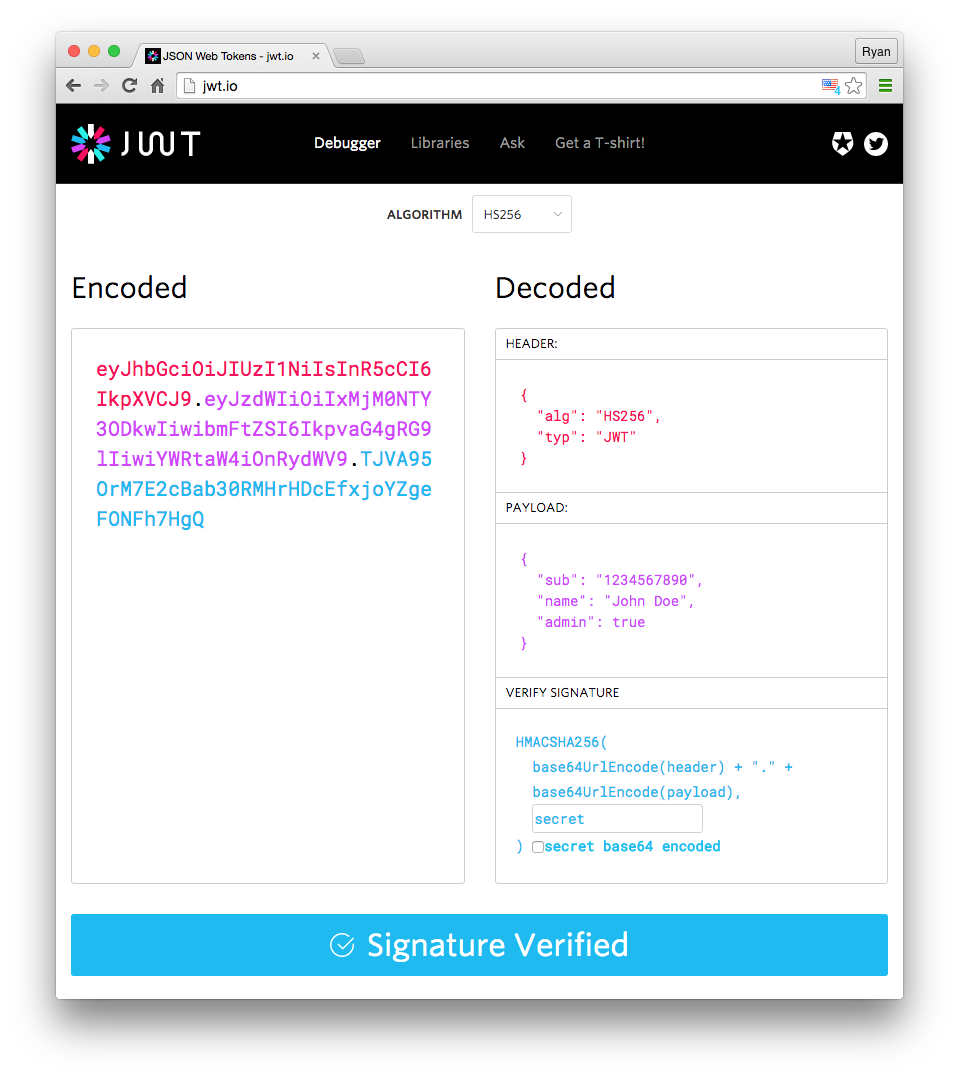
\includegraphics[width=\linewidth]{legacy-app-auth-5} 
                \caption{JWT \cite{jwtImage}}
            \end{figure}
            
            JWT se skládá ze 3 částí:
            \begin{itemize}
                \item Header
                    
                    obsahuje typ tokenu a šifrovací algoritmus.
                \item Payload
                    
                    obsahuje naše informace a může obsahovat ještě dodatečné informace jako expirace tokenu, vydavatel atd. % vydavatel = issuer
                \item Signature
                    
                    obsahuje zakódované předešlé části a secret -- náš tajný klíč.
            \end{itemize}
             V naší aplikaci využijeme tuto technologii pro ověřování totožnosti uživatelů. Naše aplikace vytvoří JWT po přihlášení a uživatel se jím bude nadále identifikovat. \cite{jwt}
            \begin{figure}[h!]
                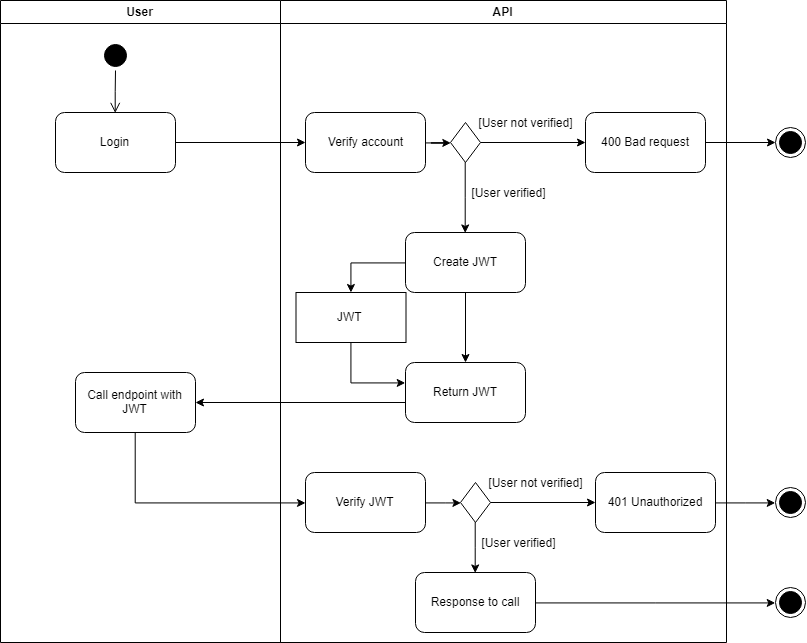
\includegraphics[width=\linewidth]{Process_of_authentication}
                \caption{Proces autorizace}
            \end{figure}
        \subsection{TSLint}
            TSLint je nástroj pro statickou analýzu kódu TypeScriptu. Detekuje potencionální chyby a udržuje jednotné fomátování kódu.\cite{tslint}
        \subsection{dotenv-safe}
            Tato knihovna umožňuje pracovat s proměnnými prostředí. Proměnné prostředí budeme zapisovat do souboru .env v kořenovém adresáři a tento soubor přidáme do gitignore souboru, protože zde budou citlivé informace. Zároveň bude existovat soubor .env.example, který bude vypadat stejně jako soubor .env, jenom nebude obsahovat hodnoty proměnných. Soubor .env.example slouží jako vzor k vytvoření .env. \cite{dotenv}
        \subsection{TypeORM}
            Jak již název napovídá jedná se o objektově relační mapování, což nám umožní jednodušeji pracovat s databází. TypeORM podporuje PostgreSQL a má npm balíček, který budeme moci využít při implementaci v Node.js.
            \cite{typeorm}
        \subsection{Docker}
            Docker je nástroj, který umožnuje vytvářet a spuštět aplikace v kontejnerech. Kontejner obsahuje aplikaci i se všemi jejími závislostmi, takže zajišťuje, že aplikace v kontejneru bude fungovat na jekékoliv platformě. Naše databáze pro vývoj a testování API poběží v Dockeru.
            \cite{docker}
\chapter{Vývoj}
    V této kapitole se budu věnovat přípravě vývojového prostědí, tutoriálu jak zpovoznit REST API a implementaci funkčního prototypu.
    \section{Vývojové prostředí pro OS~Linux}  \label{vyvProstredi}
        V této sekci se budu věnovat přípravě výojářského prostředí v Node.js a popíši zde jak zprovoznit API. Stejným postupem byla provedena i \hyperref[impl]{Implementace}.
        
        Nejprve si musíme nainstalovat Node.js a správce balíčk npm.
        \begin{minted}{bash}
sudo apt install nodejs -y
sudo apt install npm -y
    \end{minted}
        V implementaci je použita verze Node.js 10.15.3 a npm 3.5.2. Vaši verzi si můžete zkontrolovat pomocí následujích příkazů.
        \begin{minted}{bash}
nodejs -v
npm -v
        \end{minted}
        Spustíme příkaz \textit{npm init -y} v adresáři, kde chceme mít náš projekt. Ten nám zde vygeneruje jednoduchý package.json. Package.json nám definuje náš projekt, obsahuje napřklad název projektu, popis, licenci, autora, závislosti na~balíčcích. Můžeme ho upravovat v textovém editoru nebo příkazy:
        \begin{minted}{bash}
npm set init.author.email "example-user@example.com"
npm set init.author.name "example_user"
npm set init.license "MIT"
        \end{minted}
        Příklad souboru package.json najdeme v elektronické příloze src/impl/package.json.
        Dále budeme instalovat balíčky. Následujícím příkazem se nám balíček stáhne i s knihovnami, na kterých závisí, do složky node\_modules a taky se nám zapíše do package.json ve fomátu \uv{název: verze}. 
        \begin{minted}{bash}
npm i "název balíčku"
        \end{minted}
        U příkazu \textit{npm i} můžeme přidat přepínač \textit{-D}, tímto označíme balíček, který není potřeba pro běh samotné aplikace, takto označíme balíčky potřebné pro vývoj a testování např. tslint (nástroj pro statickou analýzu kódu), jest (nástroj pro testování).
        Nainstalujeme si balíčky potřebné pro naší aplikaci.
        \mint{bash}|npm i express typescript dotenv-safe|
        Dále si nainstalujeme balíčky pro statické typování viz \url{https://github.com/DefinitelyTyped/DefinitelyTyped}.
        \mint{bash}|npm i -D @types/node @types/express|
    
        Vytvoříme si tsconfig.json pro konfiguraci TypeScript. Inspirovat se můžete v elektronické příloze src/impl/tsconfig.json. Dokumetaci najdete na stránce \url{https://www.typescriptlang.org/docs/handbook/tsconfig-json.html}.

        V package.json přidáme:
        \begin{minted}{json}
"scripts": {
    "start": "ts-node src/app.ts",
}
        \end{minted}
        Vytvoříme soubor v našem adresáři src/app.ts, který bude vypadat následovně.
        \begin{minted}{TypeScript}
import *as express from 'express';
import * as path from 'path';

require('dotenv-safe').config({
    path: path.resolve(__dirname, '../.env'),
    sample: path.resolve(__dirname, '../.example.env'),
  });

const app = express();

app.get('/', (req, res) => res.send('Hello World!'));
app.listen(process.env.LISTEN_ON);
        \end{minted}
        Zbýva ještě specifikovat náš port. V souboru .example.env stačí mít pouze "LISTEN\_ON".
        \begin{minted}{bash}
echo "LISTEN_ON=4000" > .example.env && cp .example.env .env
        \end{minted}
        Teď máme vše připraveno, abychom spustili naše jednoduché API s jedním koncovým bodem. Nastartujeme aplikaci, která bude poslouchat na portu 4000 příkazem:  
        \begin{minted}{bash}
npm start
        \end{minted}
        Můžeme otestovat fukčnost v Postmanu\footnote{\url{https://www.getpostman.com}}, tak že zavoláme koncový bod, který nám vrátí Hello World! Příklad na obrázku \hyperref[fig:Postman]{4.1}.
        \begin{figure}[h!]
            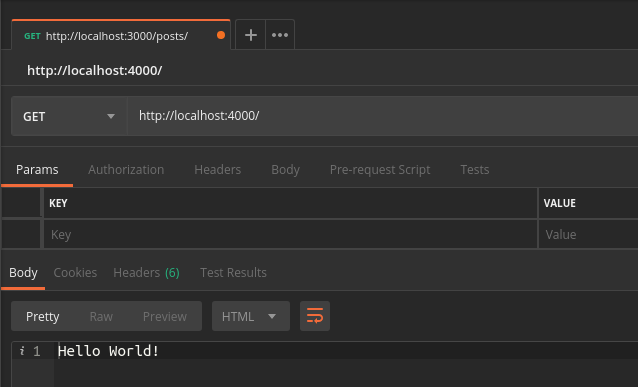
\includegraphics[width=\linewidth]{PostmanHelloWorld}
            \caption{Postman}
        \end{figure}
        \subsection{Databázové připojení s TypeORM}
            Začneme s vytvořením souboru ormconfig.json v našem kořenovém adresáři, kde bude uložena konfigurace databázového připojení. Můžete se inspirovat souborem src/impl/ormconfig.json v elektronické příloze, zde je použita PostgreSQL databáze. V této konfiguraci budeme definovat naše schéma. To zadefinujeme pomocí popsání entit. V ormconfig.json bude zapsáno, kde se naše entity nachází.
            \begin{minted}{json}
"entities": ["src/entity/**/*.ts"]
            \end{minted}
            Vytvoříme si soubor src/entity/User.ts.
            \begin{minted}{TypeScript}
import {Entity, PrimaryGeneratedColumn, Column} from "typeorm";

@Entity()
export class User {

    @PrimaryGeneratedColumn()
    id: number;

    @Column({
        unique: true,
    })
    username: string;

    @Column({
        unique: true,
    })
    email: string;

    @Column()
    password: string;

}
            \end{minted}
            Připíšeme do souboru src/app.ts vytvoření databázového připojení.
            \begin{minted}{TypeScript}
createConnection().then(async () => {
    const app = express();
    app.use(bodyParser.json());
    app.listen((process.env.LISTEN_ON && +process.env.LISTEN_ON) || 8080);
    console.log(`> Ready on http://${process.env.LISTEN_ON}`);
}).catch(error => console.log("TypeORM connection error: ", error));

            \end{minted}
            Naší databázi můžeme nechat prázdnou a TypeORM nám vytvoří schéma podle našich entit.
            Pokud máte funkční databází a správně připojení, mělo by se vám v konzoli po spuštění aplikace zobrazit:
            \begin{minted}{bash}
> Ready on http://4000
            \end{minted}
        \subsection{Volání endpointu}
            V této sekci si vytvoříme koncový bod, který nám vrátí všechny uživatele.
            
            Nejprve si vytvoříme adresář src/controller, zde se budou nacházet koncové body. Vytvoříme si zde soubor user.t, kde zadefinujeme koncový bod getAllUsers a funkci createBasicUsers, která nám vytvoří uživatele v databázi.
            \begin{minted}{TypeScript}
import {Request, Response} from "express";
import {getManager, getRepository} from "typeorm";
import { User } from '../entity/User';

export async function getAllUsers(request: Request, response: Response) {

    const postRepository = getManager().getRepository(User);

    const users = await postRepository.find();

    response.send(users);
}

function createUser(username: string, email: string, password: string): User {
    const user = new User();
    user.username = username;
    user.email = email;
    user.password = password;
    return user;
}

export async function createBasicUsers(): Promise<void> {
    await getRepository(User).save(createUser("Aman", "a@man.cz", "1234"));
    await getRepository(User).save(createUser("Batman", "batman@example.com", "1234"));
}
            \end{minted}
            Vytvoříme soubor src/routes.ts, kde se budou nacházet všechny cesty pro koncové body.
            \begin{minted}{TypeScript}
import { getAllUsers } from "./controller/user";

export const AppRoutes = [
    {
        path: "/users",
        method: "get",
        action: getAllUsers
    },
];
            \end{minted}
            Nakonec přidáme do src/app.ts následující kód, který zavolá funkci pro přidání uživatelů a přidá koncové body z src/routes.ts.
            \begin{minted}{TypeScript}
import {Request, Response} from "express";
import {AppRoutes} from "./routes";
import { createBasicUsers } from "./controller/user";

    await createBasicUsers();
    AppRoutes.forEach(route => {
        app[route.method](route.path, (request: Request, response: Response, next: Function) => {
            route.action(request, response)
                .then(() => next)
                .catch(err => next(err));
        });
    });
            \end{minted}
            Nastartujeme naší aplikaci a funkčnost můžeme otestovat v Postmanu\footnote{\url{https://www.getpostman.com}}. Zavolání koncového bodu by mělo vypadat tak, jak je zachyceno na obrázku \hyperref[fig:PostmanUsers]{4.2}.
        \begin{figure}[h!]
            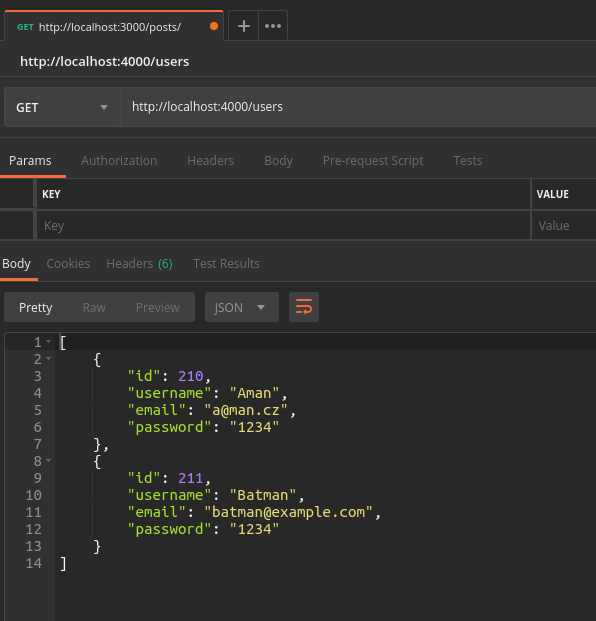
\includegraphics[width=\linewidth]{postmanUsers}
            \caption{PostmanUsers}
        \end{figure}
    \newpage
    \section{Implementace} \label{impl}
        Zde popíši jak vypadá prototyp Rest API pro editor virtuální reality. Jeho instalační příručku najdete v elektronické příloze src/impl/README.md. Naše implementace navazuje na předchozí sekci \hyperref[vyvProstredi]{Vývojové prostředí pro OS Linux}.
        
        Struktura adresáře implementace je zachycena na \hyperref[fig:adresar]{obrázku 4.3}.
        \begin{figure}[h!]
        	\dirtree{%
        		.1 docker-compose.yml\DTcomment{soubor pro spuštění databáze v Dockeru}.
        		.1 src.
        		.2 controller\DTcomment{akce koncových bodů}.
        		.2 entity\DTcomment{databázové schéma}.
        		.2 app.ts\DTcomment{hlavní spustitelný soubor}.
        		.2 routes.ts\DTcomment{specifikace URI koncových bodů}.
        		.1 .example.env\DTcomment{názvy proměnných prostředí}.
        		.1 .gitignore\DTcomment{ignorované soubory pro verzování}.
        		.1 .gitlab-ci.yml\DTcomment{skript pro GitLab CI}.
        		.1 ormconfig.json\DTcomment{připojení na databázi}.
        		.1 package.json\DTcomment{definování projektu a jeho závislostí}.
        		.1 .prettierrc\DTcomment{nastavení formátování}.
        		.1 README.md\DTcomment{instalační příručka}.
        		.1 tsconfig.json\DTcomment{konfigurace TypeScriptu}.
        		.1 tslint.json\DTcomment{nastavení linteru}.
        	}
            \label{fig:adresar}
            \caption{Adresář implementace}
        \end{figure}

		Zaměřil jsem se na nejpodstatnější část pro funkčnost editoru virtuální reality a tím je předávání grafických modelů, správa projektů a umisťování modelů do projektů.
		Práva by se musela řešit ke každému koncovému bodu a to vyžaduje rozsáhlejší analýzu. Práva v implementaci tedy řeším tak, že existuje koncový bod \textit{login}, který vrací \hyperref[jwt]{JWT}, jež expiruje po 4 hodinách od vytvoření. Tímto tokenem se uživatel bude autorizovat při volání zbylých koncových bodů.
		Znamená to tedy, že pokud se uživatel přihlásí, tak je oprávněn ke všem akcím.

        Pro tvorbu databázového schématu jsem vyšel z doménového modelu zachyceném na \hyperref[fig:domainModel]{obrázku 3.3}. Neimplementoval jsem pouze entitu Permission, z~výše zmíněného důvodu.

        Implementovány jsou koncové body pro CRUD operace entit Model, Project a Field. A k nim již zmíněný login.
        
		
		Fukční prototyp splňuje požadavky editoru virtuální reality až na spávu práv.
		Spávu práv a uživatelských účtů pro REST API si dokáži představit, jako samostatnou bakalářskou práci.
\chapter{Testování}
    Pro ověření funkčnosti našeho prototypu provedeme integrační testování. Integrační testování v našem případě vypadá jako sled volání koncových bodů (např. přihlaš se, vytvoř model, změň model, vymaž model). Pro testování našeho API použijeme testovací framework Jest\footnote{https://jestjs.io} a npm modul Axios\footnote{https://github.com/axios/axios} pro vytváření HTTP požadavků. Zavolání jednoho koncového bodu v testování vypadá následovně:
    \begin{minted}{typescript}
const secret = process.env.JWT_SECRET || '';
it('should response with 200', async () => {
  await axios({
    method: 'post',
    url: 'http://localhost:4000/login',
    data: {
      username: 'Batman',
      password: '1234',
    },
  })
    .then(response => {
      expect(typeof jwt.verify(response.data, secret)).toBe('object');
      expect(response.status).toBe(200);
    })
    .catch(error => {
      throw error;
    });
});
    \end{minted}

    Všechny testy můžeme najít v elektronické příloze src/impl/src/controller/\_\_tests\_\_.

    \section{Jest}
        Jest je framework pro testování JavaScriptových apilkací. Hodí se pro testování Node.js a typescriptu.
        Pro náš prototyp jsem vytvořil dva konfigurační soubory pro testování, které se liší pouze tím, že v jednom je navíc pokrytí kódu testy. Testy bez pokrytí se pouští příkazem:
            \begin{minted}{bash}
npm test
            \end{minted}
        A testy s pokrytím:
            \begin{minted}{bash}
npm run test-with-coverage
            \end{minted}
        Pokrytí kódu testy se nám uloží do složky coverage. V internetovém prohlížeči si můžeme otevřít soubor
        src/impl/coverage/lcov-report/index.html, který najdete v elektronické příloze, jeho podoba je zachycena na obrázku \hyperref[coverage]{5.1}.
        \begin{figure}[h!] \label{coverage}
            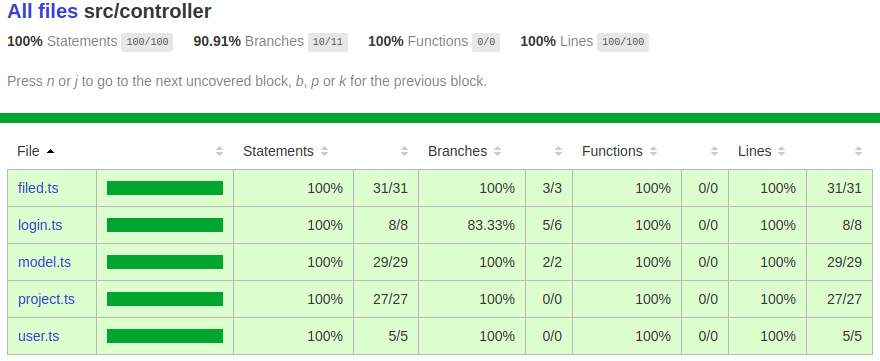
\includegraphics[width=\linewidth]{coverage}
            \caption{Pokrytí kódu testy}
        \end{figure}
        \newline
        Uvidíme v něm statistiku pokrytí kódu testy a můžeme si interaktivně procházet adresář a dívat se na pokrytí konkrétních souborů.
    \section{GitLab}
        Pro verzování teoretické i praktické části jsem používal GitLab. GitLab nabízí nástroj pro průběžnou integraci, který při každém commitu nahraném na GitLab spustí skript, který je zapsaný v souboru pojmenovaném .gitlab.yml uloženém v kořenovém adresáři projektu. Naše aplikace se po nahrání na GitLab nainstaluje a sestaví.

\begin{conclusion}
    V první části teoretické práce (analýze) proběhla analýza funkčních a nefunkčních požadavků editoru virtuální reality. Funkční požadavky byly vytvořeny ve spolupráci s Patrikem Křepinským, který momentálně pracuje na editoru virtuální reality.
	Dále byl vybrán nástroj Swagger jakožto nástroj pro návrh a dokumentaci REST API. V tomto výběru byla provedena analýza čtyř nástrojů pro návrh API a zavedení výběrové metodiky, kterou byly nástroje ohodnoceny.
	
	
	V druhé části teoretické práce (návrhu) byl proveden návrh REST API. V návrhu se vyskytl problém, že současná databáze Věnných měst českých královen nepostačuje požadavkům editoru virtuální reality, byl tedy proveden nový návrh databáze. Nakonec byly popsány technologie použité ve vývoji.
	
	
	První část praktické práce (vývoji) obsahuje popstup vývoje API v Node.js, který může být inspirací budoucím řešitelům implementace API v Node.js. Nakonec byla provedena implementace funkčního prototypu API na základě předešlého návrhu.
	
	
	V druhé části praktické práce (testování) byly naimplementovány integrační testy pro náš prototyp. Všechny testy proběhly úspěšně. Dále je zde popsané GitLab CI, které bylo využito při verzování této práce.

    % Zaobirat se cilem prakticke casti, dale lze napsat: aplikace by mohla....
\end{conclusion}

\bibliographystyle{csn690}
\bibliography{mybibliographyfile}

\appendix

\chapter{Seznam použitých zkratek}
% \printglossaries
\begin{description}
	\item[API] Application Programming Interface
	\item[CI] Continuous Integration
	\item[IDE] Integrated Development Environment
	\item[I/O] Input/Output
	\item[JSON] JavaScript Object Notation
	\item[npm] Node.js package manager
\end{description}


% % % % % % % % % % % % % % % % % % % % % % % % % % % % 
% % Tuto kapitolu z výsledné práce ODSTRAŇTE.
% % % % % % % % % % % % % % % % % % % % % % % % % % % % 
% 
% \chapter{Návod k~použití této šablony}
% 
% Tento dokument slouží jako základ pro napsání závěrečné práce na Fakultě informačních technologií ČVUT v~Praze.
% 
% \section{Výběr základu}
% 
% Vyberte si šablonu podle druhu práce (bakalářská, diplomová), jazyka (čeština, angličtina) a kódování (ASCII, \mbox{UTF-8}, \mbox{ISO-8859-2} neboli latin2 a nebo \mbox{Windows-1250}). 
% 
% V~české variantě naleznete šablony v~souborech pojmenovaných ve formátu práce\_kódování.tex. Typ může být:
% \begin{description}
% 	\item[BP] bakalářská práce,
% 	\item[DP] diplomová (magisterská) práce.
% \end{description}
% Kódování, ve kterém chcete psát, může být:
% \begin{description}
% 	\item[UTF-8] kódování Unicode,
% 	\item[ISO-8859-2] latin2,
% 	\item[Windows-1250] znaková sada 1250 Windows.
% \end{description}
% V~případě nejistoty ohledně kódování doporučujeme následující postup:
% \begin{enumerate}
% 	\item Otevřete šablony pro kódování UTF-8 v~editoru prostého textu, který chcete pro psaní práce použít -- pokud můžete texty s~diakritikou normálně přečíst, použijte tuto šablonu.
% 	\item V~opačném případě postupujte dále podle toho, jaký operační systém používáte:
% 	\begin{itemize}
% 		\item v~případě Windows použijte šablonu pro kódování \mbox{Windows-1250},
% 		\item jinak zkuste použít šablonu pro kódování \mbox{ISO-8859-2}.
% 	\end{itemize}
% \end{enumerate}
% 
% 
% V~anglické variantě jsou šablony pojmenované podle typu práce, možnosti jsou:
% \begin{description}
% 	\item[bachelors] bakalářská práce,
% 	\item[masters] diplomová (magisterská) práce.
% \end{description}
% 
% \section{Použití šablony}
% 
% Šablona je určena pro zpracování systémem \LaTeXe{}. Text je možné psát v~textovém editoru jako prostý text, lze však také využít specializovaný editor pro \LaTeX{}, např. Kile.
% 
% Pro získání tisknutelného výstupu z~takto vytvořeného souboru použijte příkaz \verb|pdflatex|, kterému předáte cestu k~souboru jako parametr. Vhodný editor pro \LaTeX{} toto udělá za Vás. \verb|pdfcslatex| ani \verb|cslatex| \emph{nebudou} s~těmito šablonami fungovat.
% 
% Více informací o~použití systému \LaTeX{} najdete např. v~\cite{wikilatex}.
% 
% \subsection{Typografie}
% 
% Při psaní dodržujte typografické konvence zvoleného jazyka. České \uv{uvozovky} zapisujte použitím příkazu \verb|\uv|, kterému v~parametru předáte text, jenž má být v~uvozovkách. Anglické otevírací uvozovky se v~\LaTeX{}u zadávají jako dva zpětné apostrofy, uzavírací uvozovky jako dva apostrofy. Často chybně uváděný symbol "{} (palce) nemá s~uvozovkami nic společného.
% 
% Dále je třeba zabránit zalomení řádky mezi některými slovy, v~češtině např. za jednopísmennými předložkami a spojkami (vyjma \uv{a}). To docílíte vložením pružné nezalomitelné mezery -- znakem \texttt{\textasciitilde}. V~tomto případě to není třeba dělat ručně, lze použít program \verb|vlna|.
% 
% Více o~typografii viz \cite{kobltypo}.
% 
% \subsection{Obrázky}
% 
% Pro umožnění vkládání obrázků je vhodné použít balíček \verb|graphicx|, samotné vložení se provede příkazem \verb|\includegraphics|. Takto je možné vkládat obrázky ve formátu PDF, PNG a JPEG jestliže používáte pdf\LaTeX{} nebo ve formátu EPS jestliže používáte \LaTeX{}. Doporučujeme preferovat vektorové obrázky před rastrovými (vyjma fotografií).
% 
% \subsubsection{Získání vhodného formátu}
% 
% Pro získání vektorových formátů PDF nebo EPS z~jiných lze použít některý z~vektorových grafických editorů. Pro převod rastrového obrázku na vektorový lze použít rasterizaci, kterou mnohé editory zvládají (např. Inkscape). Pro konverze lze použít též nástroje pro dávkové zpracování běžně dodávané s~\LaTeX{}em, např. \verb|epstopdf|.
% 
% \subsubsection{Plovoucí prostředí}
% 
% Příkazem \verb|\includegraphics| lze obrázky vkládat přímo, doporučujeme však použít plovoucí prostředí, konkrétně \verb|figure|. Například obrázek \ref{fig:float} byl vložen tímto způsobem. Vůbec přitom nevadí, když je obrázek umístěn jinde, než bylo původně zamýšleno -- je tomu tak hlavně kvůli dodržení typografických konvencí. Namísto vynucování konkrétní pozice obrázku doporučujeme používat odkazování z~textu (dvojice příkazů \verb|\label| a \verb|\ref|).
% 
% \begin{figure}\centering
% 	
\includegraphics[width=0.5\textwidth, angle=30]{cvut-logo-bw}
% 	\caption[Příklad obrázku]{Ukázkový obrázek v~plovoucím prostředí}\label{fig:float}
% \end{figure}
% 
% \subsubsection{Verze obrázků}
% 
% % Gnuplot BW i barevně
% Může se hodit mít více verzí stejného obrázku, např. pro barevný či černobílý tisk a nebo pro prezentaci. S~pomocí některých nástrojů na generování grafiky je to snadné.
% 
% Máte-li například graf vytvořený v programu Gnuplot, můžete jeho černobílou variantu (viz obr. \ref{fig:gnuplot-bw}) vytvořit parametrem \verb|monochrome dashed| příkazu \verb|set term|. Barevnou variantu (viz obr. \ref{fig:gnuplot-col}) vhodnou na prezentace lze vytvořit parametrem \verb|colour solid|.
% 
% \begin{figure}\centering
% 	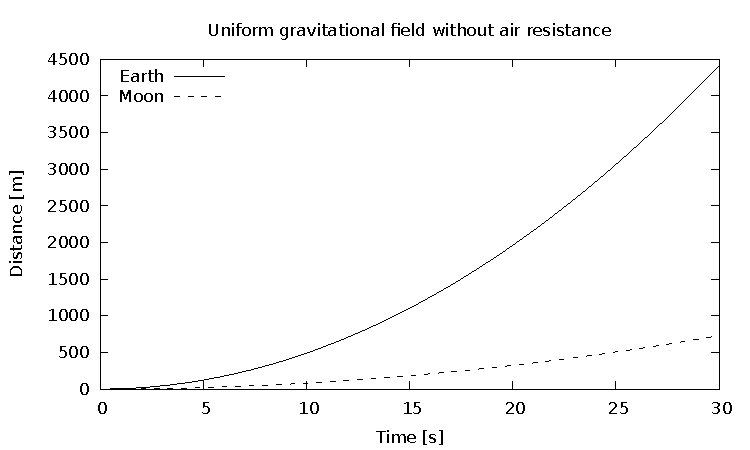
\includegraphics{gnuplot-bw}
% 	\caption{Černobílá varianta obrázku generovaného programem Gnuplot}\label{fig:gnuplot-bw}
% \end{figure}
% 
% \begin{figure}\centering
% 	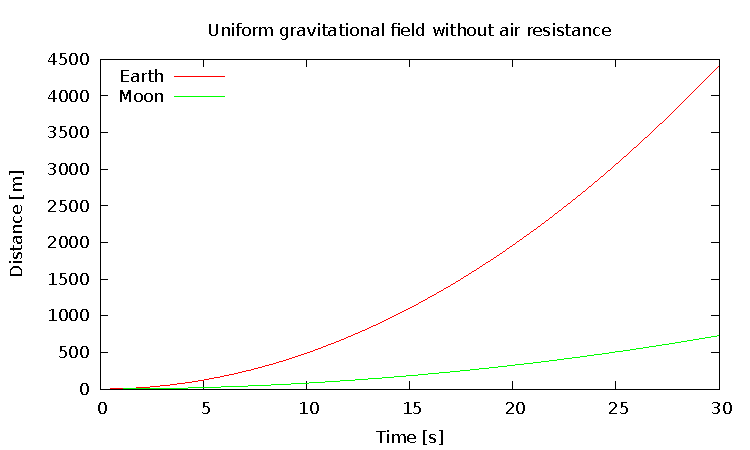
\includegraphics{gnuplot-col}
% 	\caption{Barevná varianta obrázku generovaného programem Gnuplot}\label{fig:gnuplot-col}
% \end{figure}
% 
% 
% \subsection{Tabulky}
% 
% Tabulky lze zadávat různě, např. v~prostředí \verb|tabular|, avšak pro jejich vkládání platí to samé, co pro obrázky -- použijte plovoucí prostředí, v~tomto případě \verb|table|. Například tabulka \ref{tab:matematika} byla vložena tímto způsobem.
% 
% \begin{table}\centering
% 	\caption[Příklad tabulky]{Zadávání matematiky}\label{tab:matematika}
% 	\begin{tabular}{|l|l|c|c|}\hline
% 		Typ		& Prostředí		& \LaTeX{}ovská zkratka	& \TeX{}ovská zkratka	\tabularnewline \hline \hline
% 		Text		& \verb|math|		& \verb|\(...\)|	& \verb|$...$|		\tabularnewline \hline
% 		Displayed	& \verb|displaymath|	& \verb|\[...\]|	& \verb|$$...$$|	\tabularnewline \hline
% 	\end{tabular}
% \end{table}
% 
% % % % % % % % % % % % % % % % % % % % % % % % % % % % 

\chapter{Obsah přiloženého CD}

%upravte podle skutecnosti

\begin{figure}
	\dirtree{%
		.1 readme.txt\DTcomment{stručný popis obsahu CD}.
		.1 docs\DTcomment{adresář se Swaggger dokumentací}.
		.1 src.
		.2 impl\DTcomment{zdrojové kódy implementace}.  
		.2 thesis\DTcomment{zdrojová forma práce ve formátu \LaTeX{}}.
		.1 text\DTcomment{text práce}.
		.2 thesis.pdf\DTcomment{text práce ve formátu PDF}.
	}
\end{figure}

\end{document}
